\scanpage{46}
\mspage{- IV-977 -23-}

\unsure{ïncide} avec le module de différentielles analytiques défini dans (18.13.1) ; \deleted{\illegible{4}} \inserted{en effet} (les définitions étant celles de (18.13.1)), il résulte du fait que $\overline{\Omega}^{1}_{A/k}$ est de type fini \deleted{\illegible{1}} et de (\uline{0},20.4.8) que \deleted{\illegible{12}} la dérivation $\overline{d}_{A/k}$ se factorise en \deleted{\illegible{3}} $A\xrightarrow{d_{A/k}}\Omega^1_{A/k}\xrightarrow{u_0}\overline{\Omega}^1_{A/k}$ et que tout A-homomorphisme \deleted{\illegible{1}} $\Omega^1_{A/k}\xrightarrow{u}L$, où L est un A-module de type fini, se factorise nécessairement en $\Omega^1_{A/k}\xrightarrow{u_0}\overline{\Omega}^1_{A/k}\xrightarrow{v}L$, si bien que $\operatorname{Ker}(u)$ contient toujours $\operatorname{Ker}(u_0)$, d'où notre assertion.

On notera que \uline{si} $\overline{\Omega}^1_{B/A}$ est un B-module \uline{de type fini}, il \uline{représente} le foncteur covariant $L\rightsquigarrow\operatorname{Dér}_A(B,L)$ dans la catégorie des B-modules \uline{de type fini}. \deleted{\illegible{4}} Il est clair que si $\Omega^1_{B/A}$ lui-même est \uline{de type fini} (ce qui sera par exemple le cas (\uline{0},20.4.7) lorsque B est une A-algèbre \uline{de type fini}), on a $\overline{\Omega}^1_{B/A}=\Omega^1_{B/A}$.

\uline{Proposition} (18.13.5).-- \uline{Soient} A \uline{un anneau topologique}, \deleted{\illegible{2}} \inserted{B \uline{et} C \uline{deux}} \uline{A-algèbres topologiques qui} \deleted{\illegible{1}} \inserted{\uline{sont des}} \uline{anneaux} \deleted{\illegible{10}} \uline{semi-locaux noethériens et dont les topologies sont les topologies préadiques}, $\rho:B\to C$ \uline{un A-homomorphisme continu. Alors} :

\figure{\begin{tikzpicture}\draw (0,0.7) .. controls (1.1,0.2) and (-0.2,-0.8) .. (0.2,-0.7) .. controls (1.6,1.3) and (4.8,1.3) .. (4.9,0.6) .. controls (5.1,-0.4) and (3.7,-0.6) .. (3.3,0) .. controls (2.5,-0.4) and (2.1,-0.6) .. (1.8,-0.4);\end{tikzpicture}}

(i) \uline{Si} \deleted{\unsure{C est un B-module}\illegible{5}} $\overline{\Omega}^1_{C/A}$ \uline{est un C-module de type fini} \deleted{\illegible{1}} $\overline{\Omega}^1_{C/B}$ \uline{est un C-module de type fini}.

(ii) \uline{Si} $\overline{\Omega}^1_{B/A}$ \uline{est un B-module de type fini et si} C \uline{est une B-algèbre finie}, $\overline{\Omega}^1_{C/A}$ \uline{est un C-module de type fini}.

(iii) \uline{Supposons vérifiées, soit les hypothèses de} (ii), \uline{soit} \deleted{\illegible{2}} \uline{l'hypothèse de} (i) \uline{et la condition supplémentaire que} $\Omega^1_{B/A}$ \uline{est un B-module de type fini ; alors il existe deux C-homomorphismes} \deleted{\uline{déterminés de} \inserted{façon} \uline{unique}}, $\overline{u}:\overline{\Omega}^1_{C/A}\to\overline{\Omega}^1_{C/B}$ \uline{et} \deleted{\unsure{:}} $\overline{v}:\overline{\Omega}^1_{B/A}\otimes_B C\to\overline{\Omega}^1_{C/A}$ \uline{tels que le diagramme}
\margin{style \uline{ambigu}}
\figure{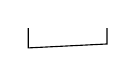
\begin{tikzpicture}\draw (0,0.2)--(0,-0.05)--(1,0)--(1,0.2);\end{tikzpicture}}

\diagram{\begin{tikzcd}[ampersand replacement=\&,column sep=large]
\Omega^1_{B/A}\otimes_B C \arrow[r,"v"] \arrow[d,"r'\otimes1"'] \& \Omega^1_{C/A} \arrow[r,"u"] \arrow[d,"r"'] \& \Omega^1_{C/B} \arrow[r] \arrow[d,"r''"] \& 0 \\
\overline{\Omega}^1_{B/A}\otimes_B C \arrow[r,"\overline{v}"'] \& \overline{\Omega}^1_{C/A} \arrow[r,"\overline{u}"'] \& \overline{\Omega}^1_{C/B} \arrow[r] \& 0
\end{tikzcd}}
\margin{(18.13.5.1)}
\margin{45}
